\chapter{Introduction}
\label{chap:intro}

More than ever we are overwhelmed by an amount of data which is created every day. When we compare how data has been created over the past years, we realize that is already increasing significantly. Besides this evolution, nowadays we have the most diverse kinds of data (e.g., documents, tweets, pictures, videos, GIFs, check-ins).

This phenomenon has been called \textit{Big Data} and represents an increasing field of study for the time being. Therefore researchers are analyzing and learning with these information we create. However the increasing amount of data make analyses hard to perform. So, people are investing in techniques and tools to tackle challenges such as data mining, data cleaning, data visualization, data classification, data exploration and so on.

One common kind of data is what we called {\em spatial data}, which are data the comes with geographical attributes like latitude and longitude (e.g., tweets, restaurants reviews, place check-ins). Spatial data can be very insightful, for instance, a check-in at the airport by your sister in the morning of your birthday, probably it means you will have a surprise.

As each record in spatial data represents an activity in a precise geographical location, analyzing such data enables discoveries grounded on facts. Analysts are often interested to observe spatial patterns and trends to improve their decision making process. Spatial data analysis has various applications such as smart city management, disaster management and autonomous transport \cite{RoddickEHPS04,Telang:2012}.

\section{Problem Definition}

Spatial data analysis is often performed in {\em exploratory context}: the analyst does not have a precise query in mind and she explores data in iterative steps in order to find potentially interesting results. Traditionally, an exploratory analysis scenario on spatial data is described as follows: the analyst visualizes a subset of data using a query in an visualization environment (e.g., Tableau\footnote{\it http://www.tableau.com},
Exhibit\footnote{\it http://www.simile-widgets.org/exhibit/},
Spotfire\footnote{\it http://spotfire.tibco.com}). The result will be illustrated on a geographical map. Then she investigates on different parts of the data by zooming in/out and panning the map in order to discover patterns and trends of interest. The analyst may iterate on this process several times by issuing different queries and focusing on different aspects of data.

The large size of spatial data make the analyst feel lost during the exploration. There could be thousands of points in each neighborhood of a city, for example. Analysts require to obtain only few options (so-called ``highlights'') to act as a direction and be able to focus on. In the perfect scenario, these options are not randomly chosen and represent what they showed to be interested in the previous iterations.

In this work, we formulate a solution for ``information highlighting using feedback collected over time'', i.e., highlight few geographical points based on interests of the analyst in order to guide the her towards what she should concentrate on in consecutive iterations of the analysis process.

\subsection{Case Study}

Now, we will present a case study in order to show the functionality of our approach in practice.

\begin{figure}[t]
	\centering
	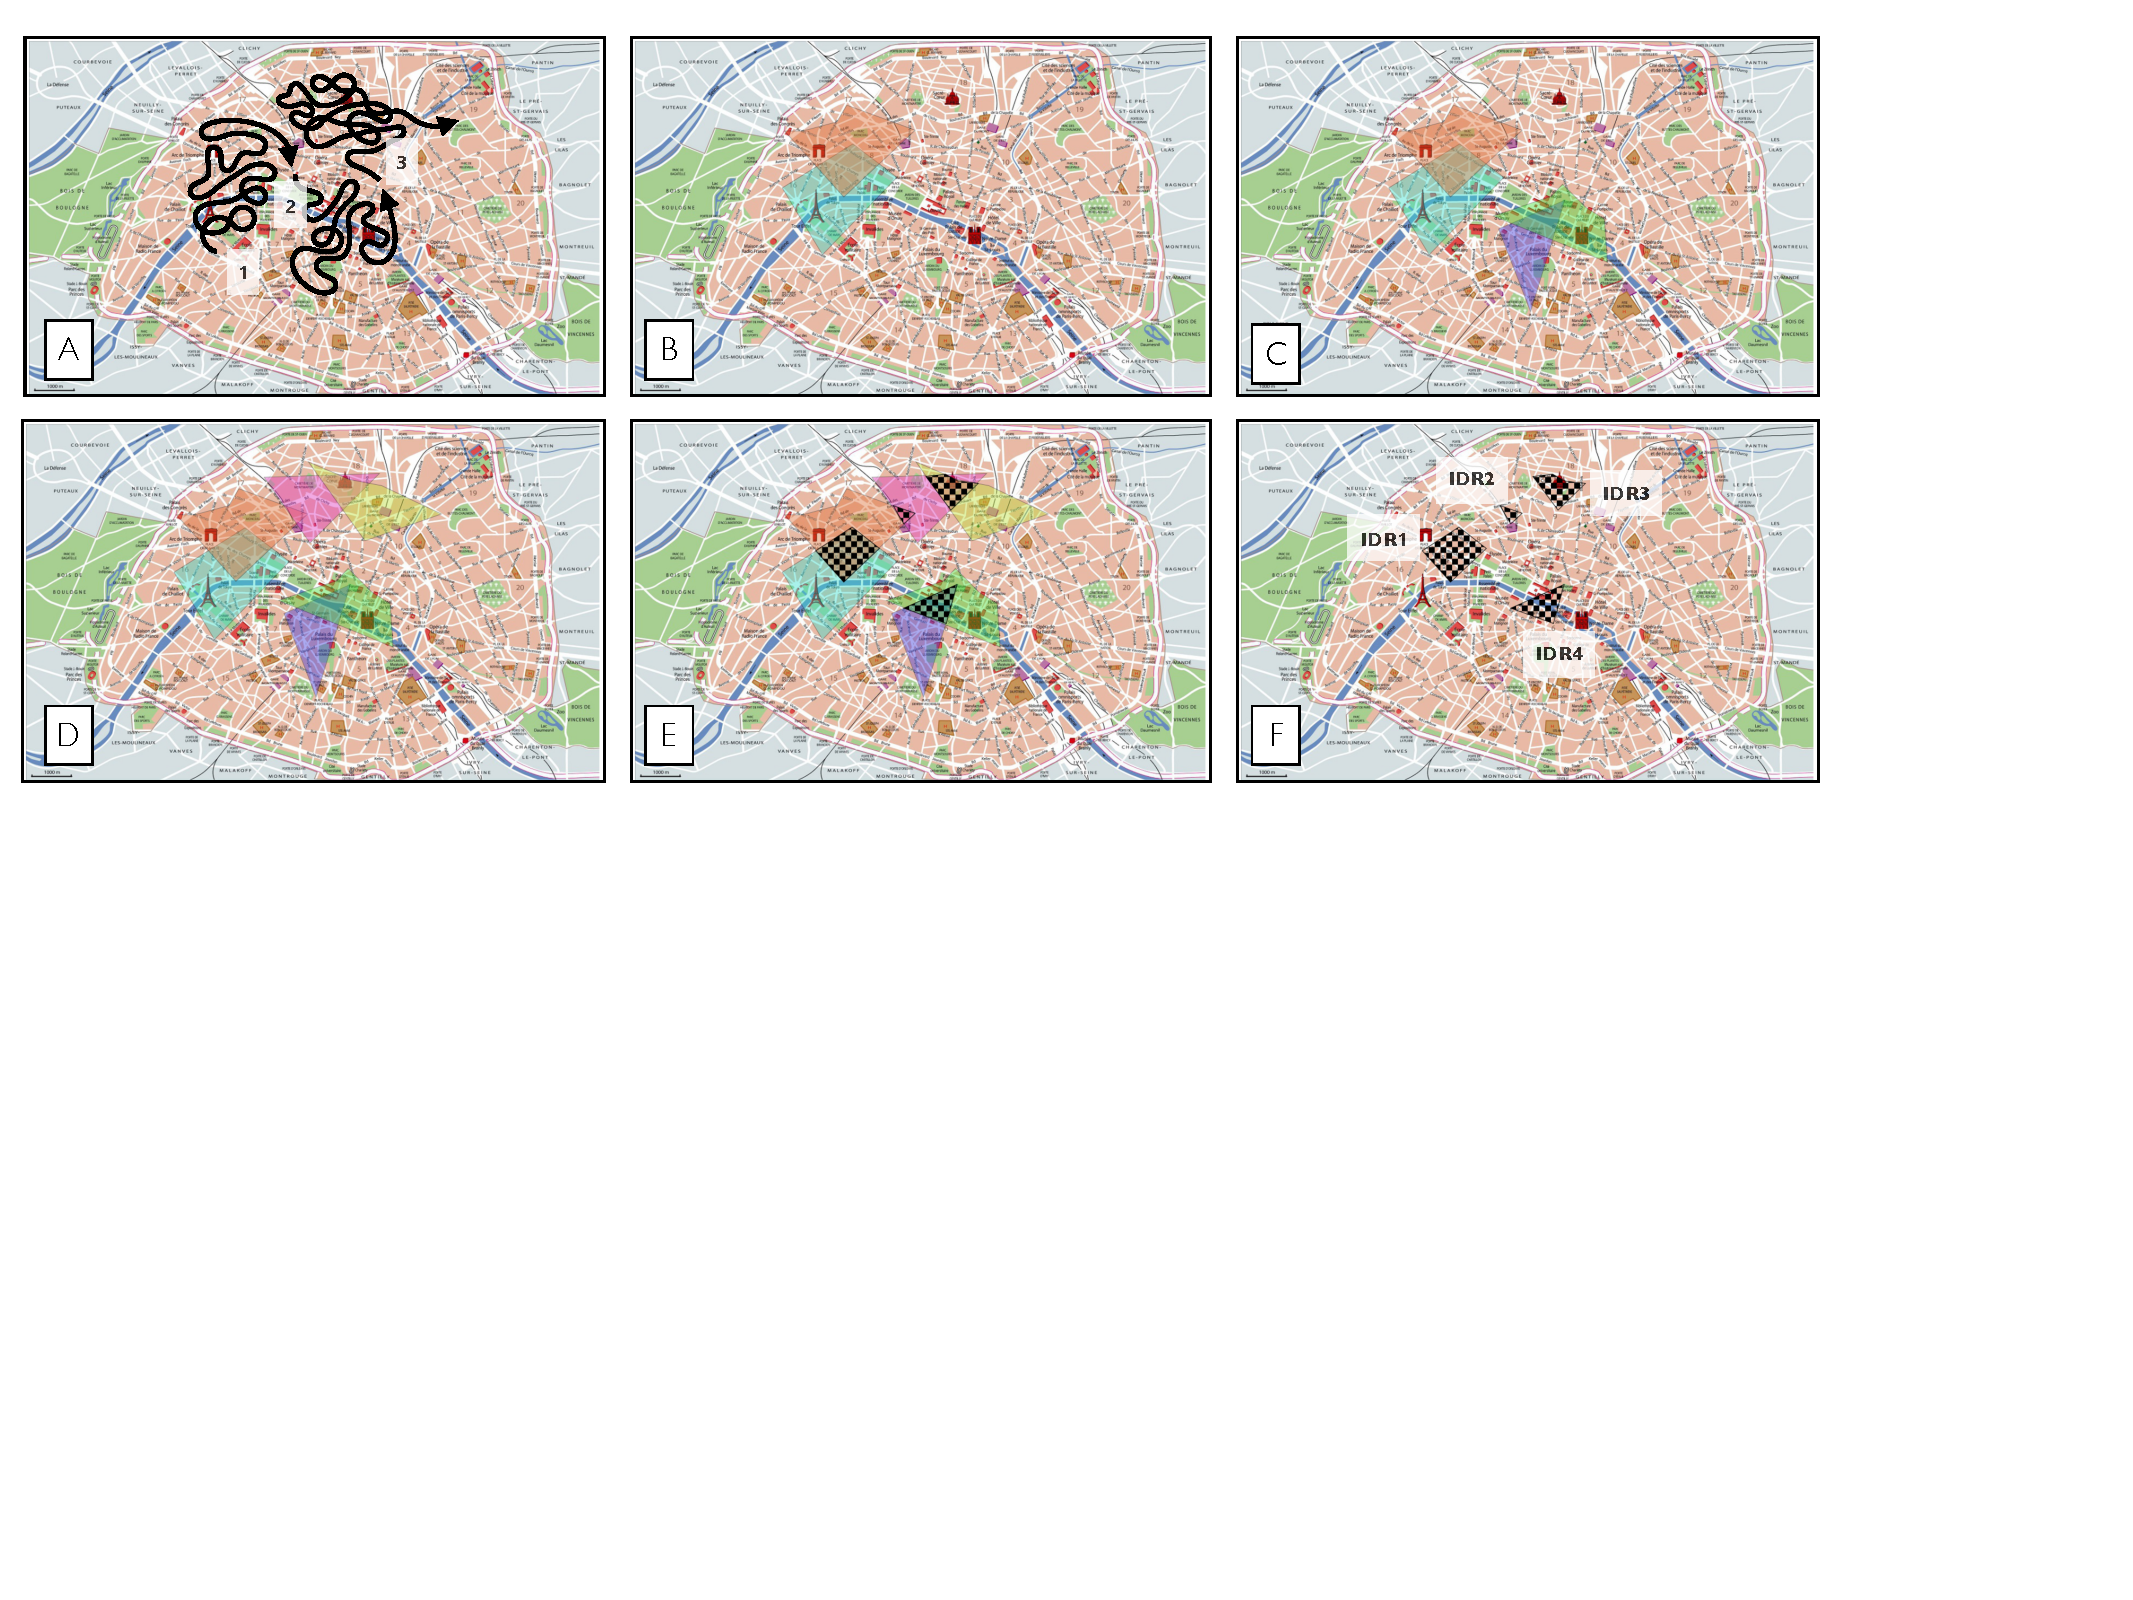
\includegraphics[width=\textwidth]{imagens/regions}
	\caption{The process of exploring Paris home-stays.}
	\label{fig:regions}
\end{figure}

{\bf Example.} {\em Lucas is planning to spend few days in Paris, France. His appreciation of French culture makes him interested in new experiences in the city. He decides to rent a home-stay from Airbnb website\footnote{\it http://www.airbnb.com}. He likes to discover the city, hence he is open to any type of lodging in any region with an interest to stay in the city center. The website returns $4000$ different locations. As he has no other preferences, an exhaustive investigation needs scanning each location independently which is nearly infeasible. While he is scanning few first options, he shows interest in the region of ``Champ de Mars'' (near Eiffel Tower), but he forgets or doesn't feel necessary to click a point there. By collecting feedback on his mouse moves over the home-stays in Paris, our system can quickly detect his interest in the region and short-list a small subset of locations (i.e., highlights) accordingly to be recommended to Lucas.}

We follow the above example to describe how implicit feedback is collected in action. Figure \ref{fig:regions} shows Lucas' steps to explore home-stays in Paris. Figure \ref{fig:regions}.A shows his mouse movements in different time stages. In this example, we consider $g = 3$ and capture Lucas' feedback in three different time segments (progressing from Figures \ref{fig:regions}.B to \ref{fig:regions}.D). It shows that Lucas started his search around Eiffel Tower and Arc de Triomphe (Figure \ref{fig:regions}.B) and gradually showed interest in south (Figure \ref{fig:regions}.C) and north (Figure \ref{fig:regions}.D) as well. All intersections between those regions are discovered (hatching regions in Figure \ref{fig:regions}.E) which will constitute the set of {\em Interesting Dense Regions} (Figure \ref{fig:regions}.F), i.e., IDR1 to IDR4.

What if Lucas wanted to come back to Paris, France next year? He will have to repeat the same exploratory analyse, unless he remember the exact location of home-stays he showed interest last year. Using our system, he won't need to remember, because his preferences were collected and can be used to highlight a subset of similar home-stays.

In the context of exploratory analysis, the analyst may change his preferences between session (e.g., in the winter, Lucas may want to be close to the Eiffel Tower, but in the summer, he may not). In order to tackle this challenge we also apply a temporal analyse to identify patterns in how the analyst preferences change between sessions which allow our highlighting method to be more precise and consistent to the analyst interest.

\section{Objectives}

In this section, we define the general and specific objectives of our work.

\subsection{General Objectives}

\begin{itemize}
	\item Introduce a time-aware guidance approach for spatial data exploration;
	\item Elaborate how temporal analyses can be effectively applied in data exploration;
\end{itemize}

\subsection{Specific Objectives}

\begin{itemize}
	\item Describe our data model used for temporal analyses;
	\item Describe our concept of {\em Interesting Dense Regions} used for collecting feedback;
	\item Present the results of our guidance approach.
\end{itemize}

\section{Organization}

The next chapters is as follow: in the Chapter \ref{chap:background} we discuss the background of this work. Chapter \ref{chap:model} defines the data model. Chapter \ref{chap:collecting} presents how the feedback is collected during exploration. Chapter \ref{chap:applying} presents how temporal analysis is applied. Chapter \ref{chap:guiding} presents how highlight interesting points in order to guide the user using collected feedback and results from temporal analysis. Chapter \ref{chap:experiments} shows experiments and its results. Chapter \ref{chap:conclusion} presents some conclusions and future directions.
